\begin{figure}[h]
    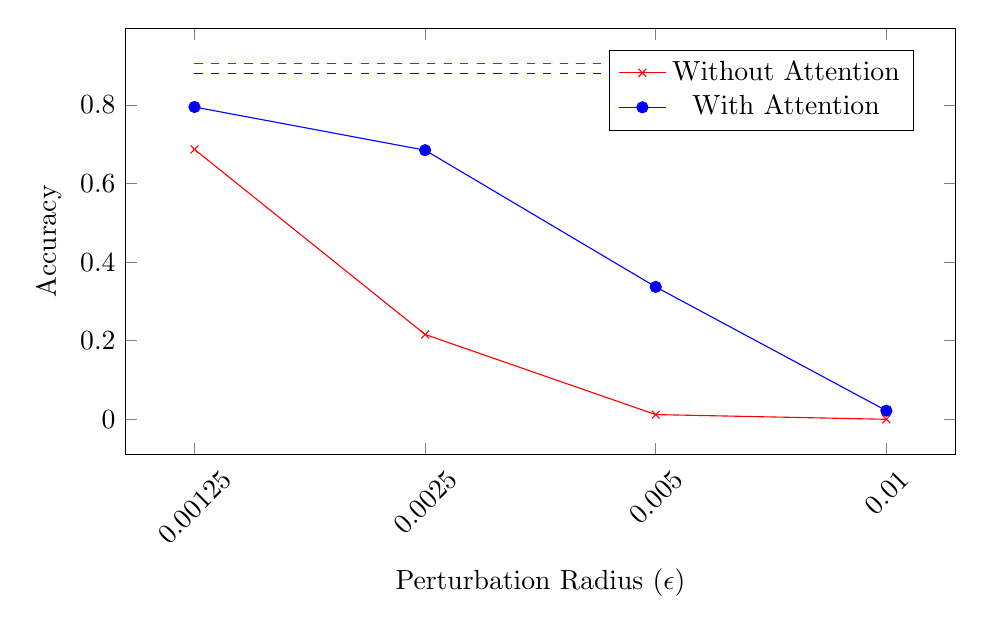
\begin{tikzpicture}
      \begin{axis}[xtick={0, 0.00125, 0.0025, 0.005, 0.01, 0.02, 0.04, 0.08, 0.16, 0.32}, x tick label style={rotate=45, log ticks with fixed point},xmode=log, log basis x=2, xlabel=Perturbation Radius ($\epsilon$), ylabel=Accuracy, width=\linewidth, height=7cm,legend style={at={(0.95,0.95)},anchor=north east}]
          
      \addplot[color=red,mark=x] coordinates {
        (0.00125, 0.687)
        (0.0025, 0.216)
        (0.005, 0.012)
        (0.01, 0)
      };
      
      \addplot[color=blue,mark=*] coordinates {
        (0.00125, 0.795)
        (0.0025, 0.685)
        (0.005, 0.337)
        (0.01, 0.022)
      };

      \addplot[color=red, domain=0.00125:0.01, dashed]{0.905};
      \addplot[color=blue, domain=0.00125:0.01, dashed]{0.880};
      
      \legend{Without Attention,With Attention}
      \end{axis}
      \end{tikzpicture}
    \caption{Clean- and robust-accuracy of ResNet-50 models for skin lesion classification.  Dashed lines represent clean-accuracy.}
    \label{DermResNet50Robustness}
  \end{figure}